\documentclass[a4paper]{article}

%% Language and font encodings
\usepackage[english]{babel}
\usepackage[utf8x]{inputenc}
\usepackage[T1]{fontenc}

%% Sets page size and margins
\usepackage[a4paper,top=3cm,bottom=2cm,left=3cm,right=3cm,marginparwidth=1.75cm]{geometry}

%% Useful packages
\usepackage{siunitx}
\usepackage{amsmath}
\usepackage{graphicx}
\usepackage{amssymb}
\usepackage[colorinlistoftodos]{todonotes}
\usepackage[colorlinks=true, allcolors=blue]{hyperref}

\graphicspath : \graphicspath{{Images/}}

\title{Code abstract}
\author{Jonathan Granier}

\begin{document}
\maketitle

This is a short abstract of the code that explain how the code work in general.

\section{Prototype abstract}

The prototype take as input \textit{DEM} files (.asc) and make a 3D render of this. The main goal is generate the shading and the shadow of the mountains and display them on a mesh. For generate the shading , the main idea is generate a multi scale with a laplacien pyramid and on each scale , locally directs the light with the slant. 




\section{Explanation of the code}
It's a OpenGL code with two parts. The C++ code (in the \textit{cpp} folders) and the shader (in \textit{shaders} folder).  

\subsection{C++}

This code is split in 2 parts. The UI in the \textit{MainWidnow} folder and the engine in the \textit{OpenGL} and \textit{LightCamera} folder.


\subsubsection{MainWindow}
The UI of the prototype. All QT code are in this folder. 

\begin{itemize}
\item main.cpp : Just start the app and run mainwindow.
\item mainwindow.cpp : Setup the UI and start viewer. Do the connection between the UI and the viewer. 
\item mainwindow.ui : A UI files generate by QTdesigner.
\item viewer.cpp : The real main class of the project. Make the link between the UI and the engine. Setup the opengl context. Controle the light , the camera and the scene. Select wich part of the pipeline will be display on the screen (Drawmode). 
\end{itemize}


\subsubsection{Light Camera}
Just vector and matrix computation for manage a camera and a light

\begin{itemize}
\item Light : Define by the 2 Euler's angle yaw and pitch. 
\item Camera and Trackball : A Camera that move around a central point. 
\end{itemize}


\subsubsection{OpenGL}



\begin{itemize}
\item Scene : Manage the multi scale, and the computation order . 
\item Scale : Manage a scale. 
\item mesh,vertex : Manage the mesh.
\item meshloader : translate a DEM to a heightMap (texture) and a heightMap to a mesh.
\item Textures : Load or generate a texture, send the texture to GPU.  
\end{itemize}





\subsubsection{Pipeline}
\begin{itemize}
\item MainWindow : UI
\item Viewer : Central point, select the texture to display
\item Scene : Manage the computation order of the multi-scale and the shared settings.
\item Scale : Manage a unique scale, uniform to send to the shaders. 
\end{itemize}



\begin{figure}
\begin{centering}
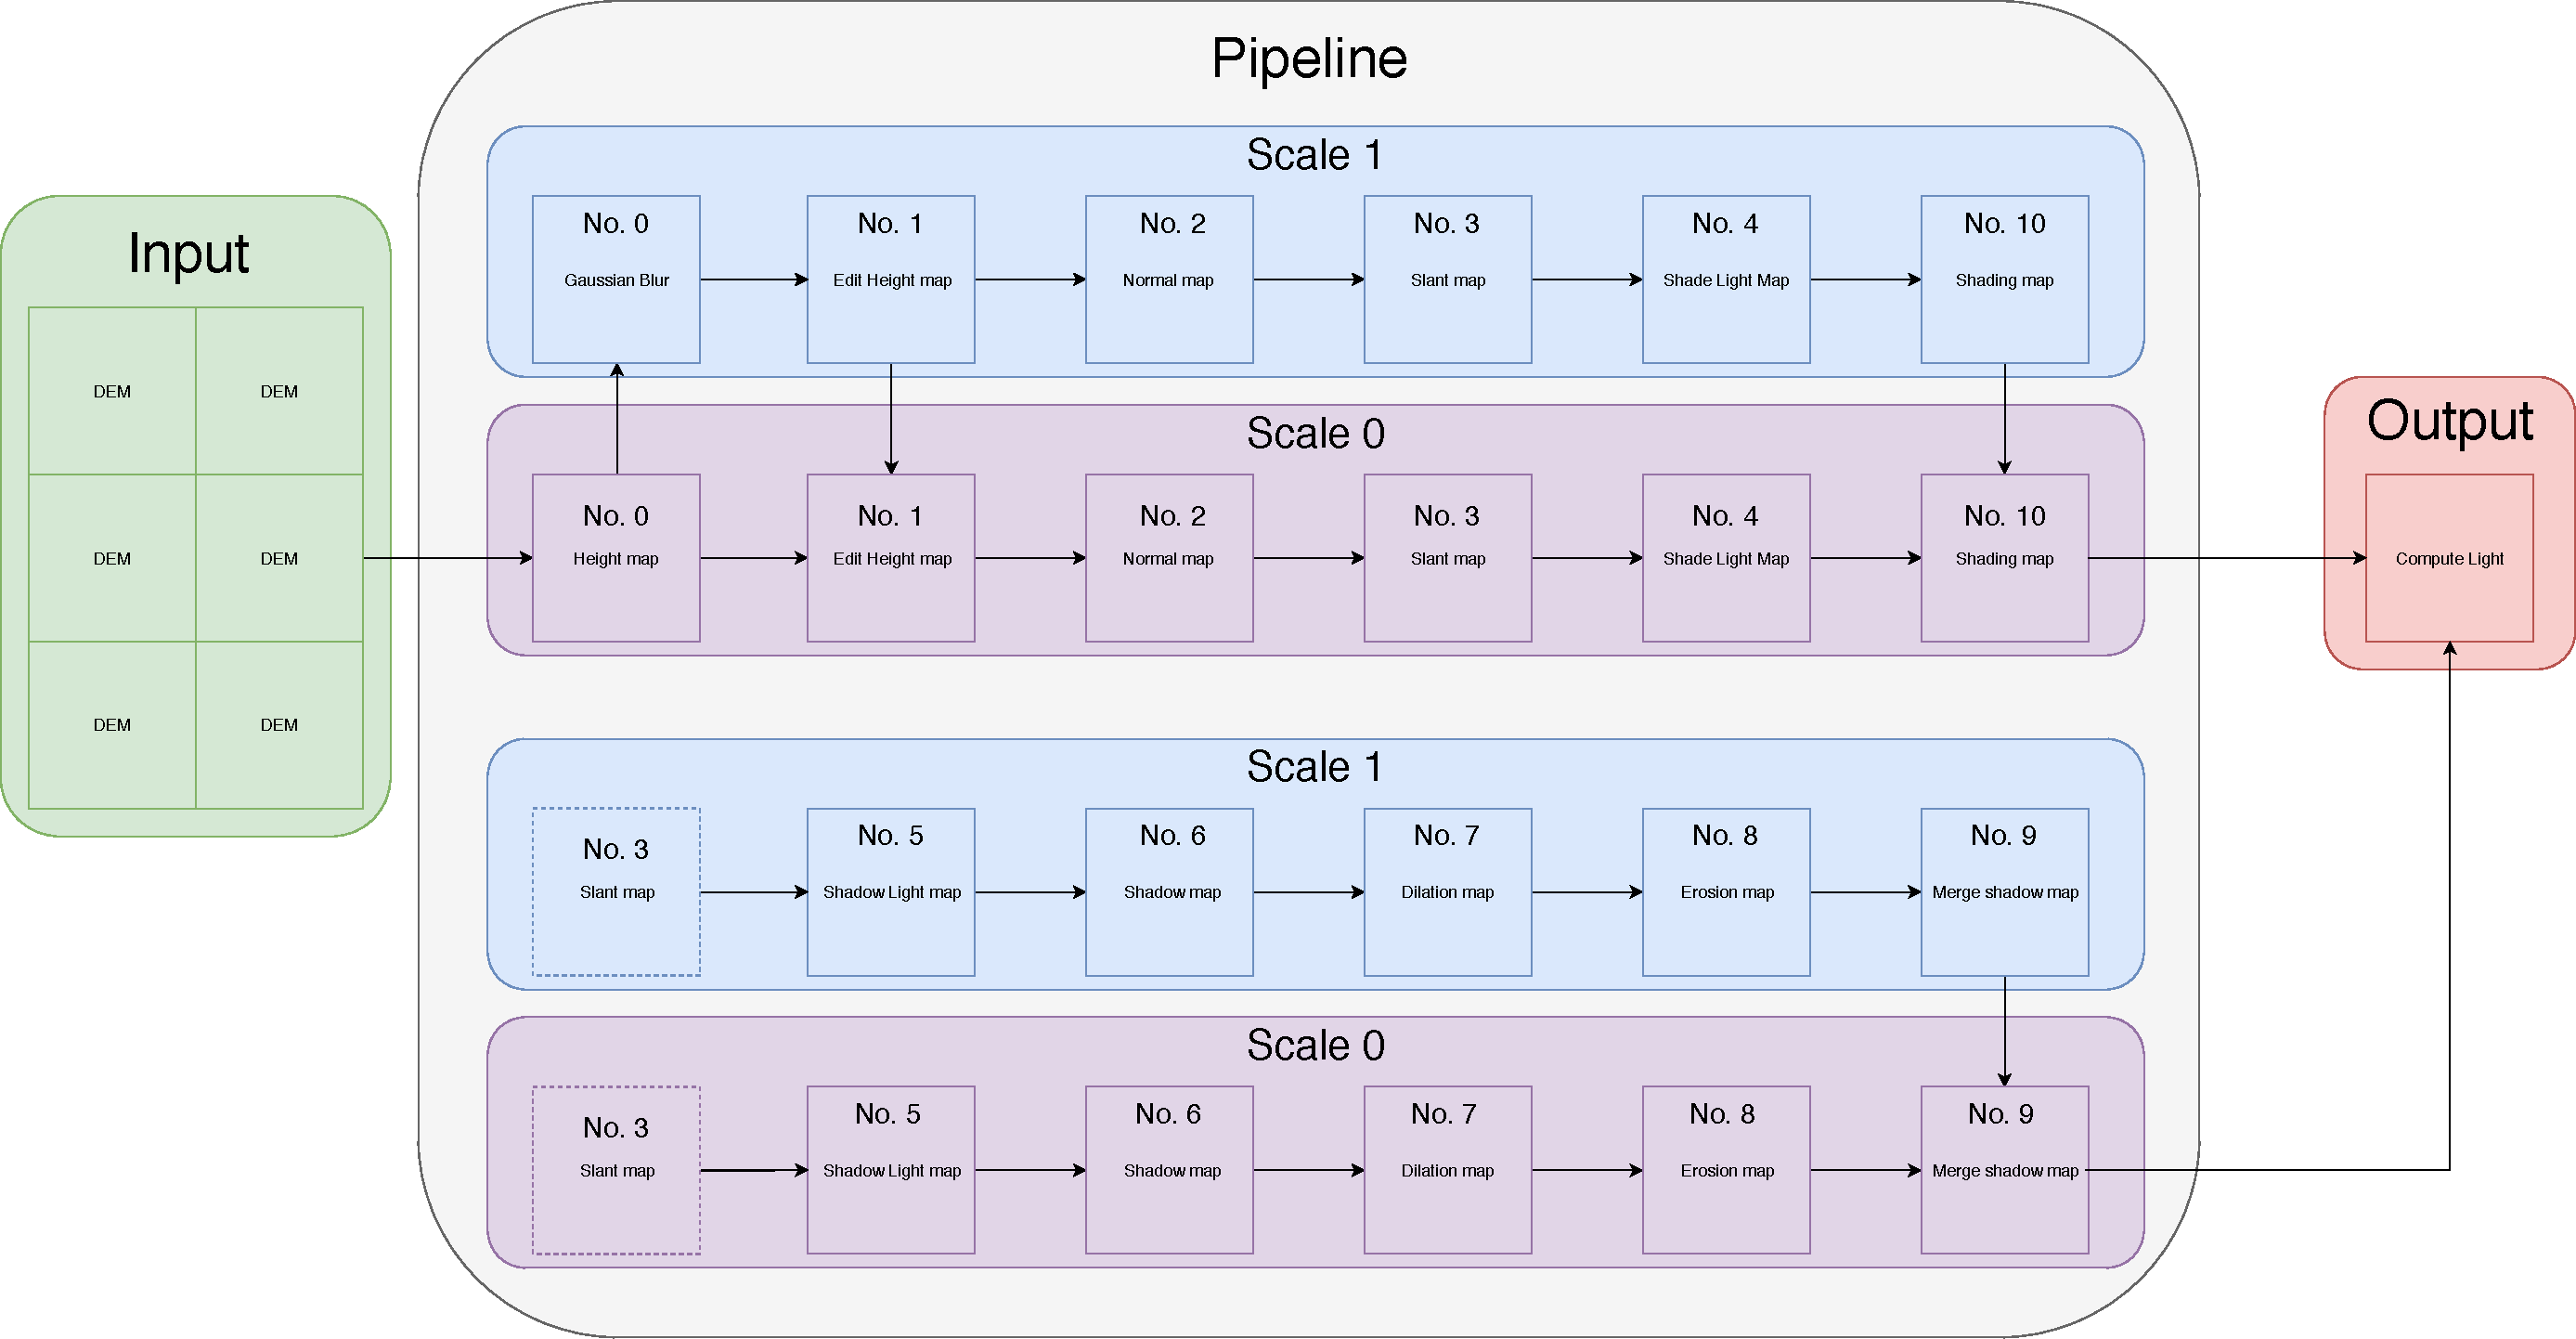
\includegraphics[scale=0.35]{../../ressources/schemas/Pipeline.pdf}
\end{centering}
\end{figure}

\subsection{Shaders}
All the computation are done in the image space. 

The shaders 
\begin{itemize}

\item No. 0. gaussBlur : Do a Gaussian blur on a height map. First part of the Laplacien pyramid.
\item No. 1. editheightmap :  Do the difference beetween two heightMap. Second part of the Laplacien pyramid.
\item No. 2. normalmap : Compute the normals of a height map.
\item No. 3. slantmap : Compute the slant map of a height Map.
\item No. 4. shadelight : Directs localy the light with the slant. Compute the light for the shading only.
\item No. 5. shadowlight : Directs localy the light with the slant. Compute the light for the shadows only.
\item No. 6. shadowmap : Compute the shadow map with a raymarching.
\item No. 7,8. morpho : Make a mathematical morphology on a shadow map.
\item No. 9. mergeshadow :  Merge two shadows maps with a lineare interpolation.
\item No. 10. shading : Compute the shading from the normalMap and the local light.
\item No. 11. ComputeLight : Only shader with the mesh. Mix the mesh with the shading , the shadows and the color
\item genheightMap : Out of the pipeline. Generate a height map in level of gray
\item drawTexture : Out of the pipeline. Shader for draw a unique texture.
\end{itemize}

The textures :
\begin{itemize}

\item No. 0. HeightMap : level of gray between 0 and 4809 (height of the \textit{Mont blanc}).
\item No. 1. EditHeightMap : level of gray between 0 and 4809( height of the \textit{Mont blanc} ).
\item No. 2. NormalMap : 3D vector , y up.
\item No. 3. SlantMap : 2D vector + size of the vector in blue chanel.
\item No. 4. ShadelightMap : 3D vector.
\item No. 5. ShadowlightMap : 3D vector.
\item No. 6. ShadowMap : Boolean value in the red chanel. 0--> shadow , 1--> no shadow. 
\item No. 7. DilationMap : Boolean value in the red chanel. 0--> shadow , 1--> no shadow. 
\item No. 8. ErosionMap : Boolean value in the red chanel. 0--> shadow , 1--> no shadow. 
\item No. 9. mergeshadowMap :  Value between 0 and 1 in red chanel.
\item No. 10. shadingMap : level of gray between 0 and 1. 
\end{itemize}
\end{document}
